\section{Labeling}

\begin{frame}{Labeling}{Feature}

\begin{columns}
\column{0.6\textwidth}
\begin{figure}
\centering
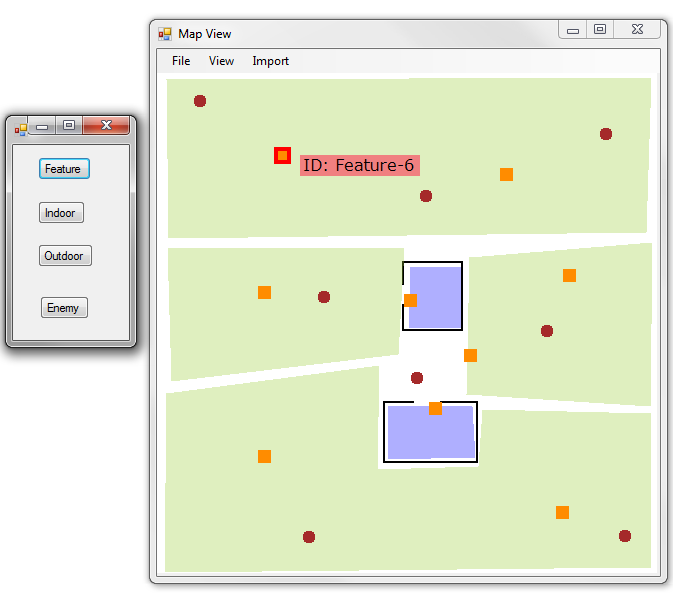
\includegraphics[width = \textwidth]{./screenshot/feature_label.png}
\end{figure}

\column{0.4\textwidth}
\begin{minipage}{\textwidth}
\begin{itemize}
\item Position
\item ID
\item Name
\end{itemize}
\end{minipage}
\end{columns}

\end{frame}

\begin{frame}{Labeling}{Indoor}

\begin{columns}
\column{0.6\textwidth}
\begin{figure}
\centering
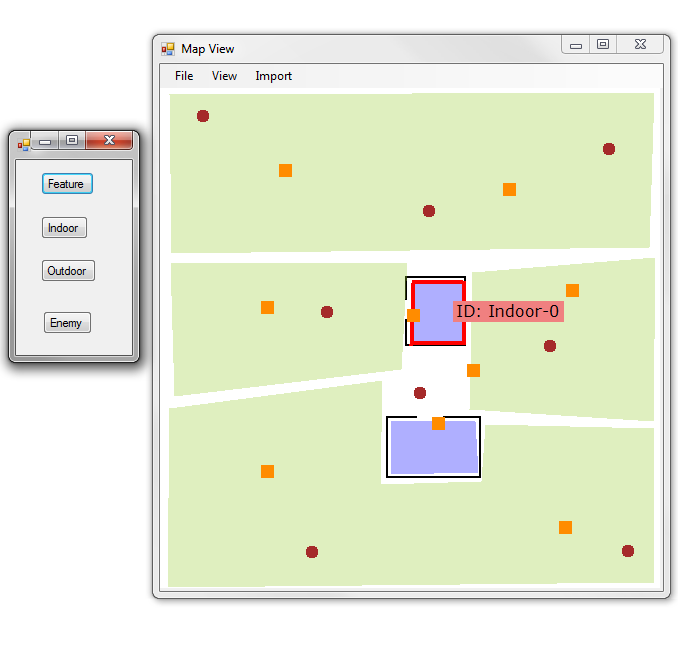
\includegraphics[width = \textwidth]{./screenshot/indoor_label.png}
\end{figure}

\column{0.4\textwidth}
\begin{minipage}{\textwidth}
\begin{itemize}
\item Vertex List
\item ID
\item Name
\end{itemize}
\end{minipage}
\end{columns}

\end{frame}

\begin{frame}{Labeling}{Outdoor}

\begin{columns}
\column{0.6\textwidth}
\begin{figure}
\centering
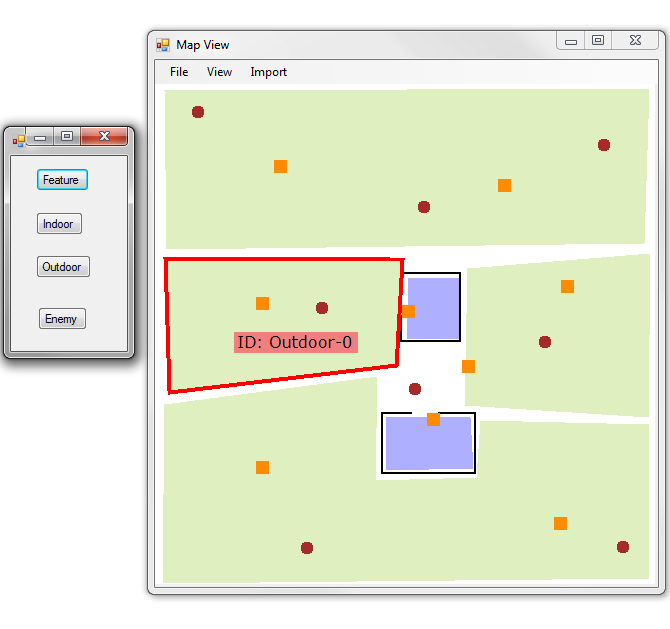
\includegraphics[width = \textwidth]{./screenshot/outdoor_label.png}
\end{figure}

\column{0.4\textwidth}
\begin{minipage}{\textwidth}
\begin{itemize}
\item Vertex List
\item ID
\item Name
\item Type
\end{itemize}
\end{minipage}
\end{columns}

\end{frame}

\begin{frame}{Labeling}{Enemy}

\begin{columns}
\column{0.6\textwidth}
\begin{figure}
\centering
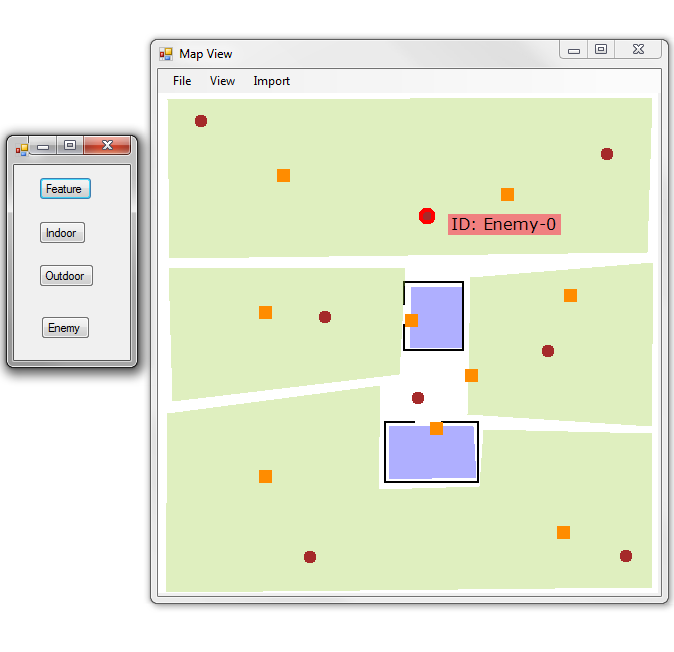
\includegraphics[width = \textwidth]{./screenshot/enemy_label.png}
\end{figure}

\column{0.4\textwidth}
\begin{minipage}{\textwidth}
\begin{itemize}
\item ID
\item Name
\item Position
\end{itemize}
\end{minipage}
\end{columns}

\end{frame}

\begin{frame}{Label data format}{XML}

\begin{columns}
\column{0.7\textwidth}
\begin{figure}
\centering
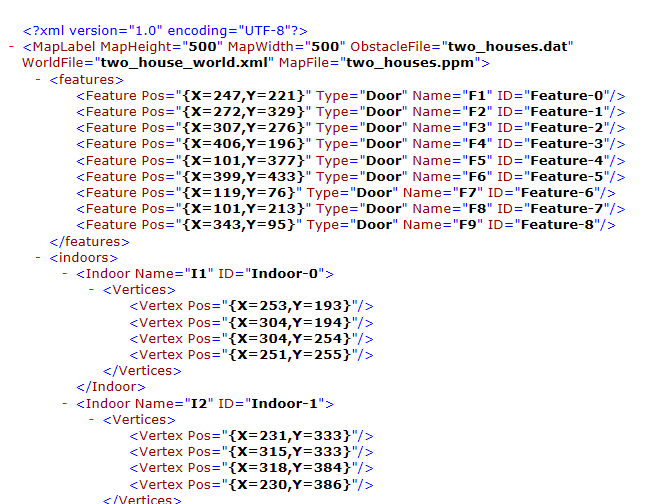
\includegraphics[width = \textwidth]{./screenshot/label_data_xml.png}
\end{figure}

\column{0.3\textwidth}
\begin{minipage}{\textwidth}
To be connected with RTCA robot perception.
\begin{figure}
\centering
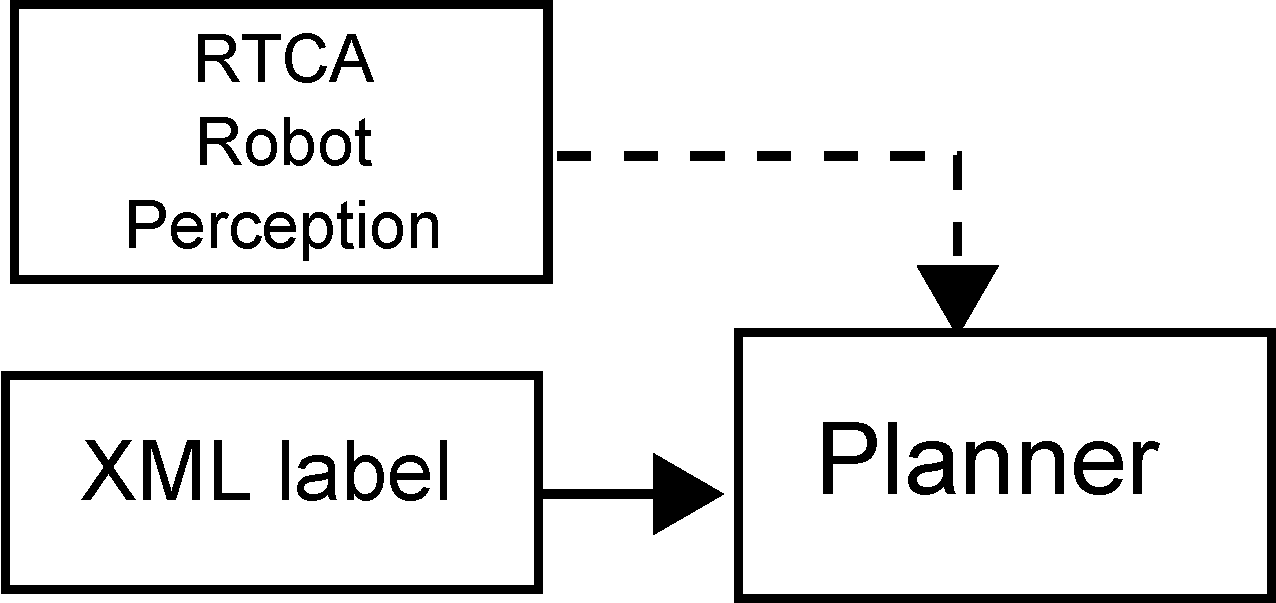
\includegraphics[width = \textwidth]{./figure/interconnect}
\end{figure}
\end{minipage}
\end{columns}

\end{frame}